% Options for packages loaded elsewhere
\PassOptionsToPackage{unicode}{hyperref}
\PassOptionsToPackage{hyphens}{url}
%
\documentclass[
]{article}
\usepackage{amsmath,amssymb}
\usepackage{lmodern}
\usepackage{iftex}
\ifPDFTeX
  \usepackage[T1]{fontenc}
  \usepackage[utf8]{inputenc}
  \usepackage{textcomp} % provide euro and other symbols
\else % if luatex or xetex
  \usepackage{unicode-math}
  \defaultfontfeatures{Scale=MatchLowercase}
  \defaultfontfeatures[\rmfamily]{Ligatures=TeX,Scale=1}
\fi
% Use upquote if available, for straight quotes in verbatim environments
\IfFileExists{upquote.sty}{\usepackage{upquote}}{}
\IfFileExists{microtype.sty}{% use microtype if available
  \usepackage[]{microtype}
  \UseMicrotypeSet[protrusion]{basicmath} % disable protrusion for tt fonts
}{}
\makeatletter
\@ifundefined{KOMAClassName}{% if non-KOMA class
  \IfFileExists{parskip.sty}{%
    \usepackage{parskip}
  }{% else
    \setlength{\parindent}{0pt}
    \setlength{\parskip}{6pt plus 2pt minus 1pt}}
}{% if KOMA class
  \KOMAoptions{parskip=half}}
\makeatother
\usepackage{xcolor}
\usepackage[margin=1in]{geometry}
\usepackage{color}
\usepackage{fancyvrb}
\newcommand{\VerbBar}{|}
\newcommand{\VERB}{\Verb[commandchars=\\\{\}]}
\DefineVerbatimEnvironment{Highlighting}{Verbatim}{commandchars=\\\{\}}
% Add ',fontsize=\small' for more characters per line
\usepackage{framed}
\definecolor{shadecolor}{RGB}{248,248,248}
\newenvironment{Shaded}{\begin{snugshade}}{\end{snugshade}}
\newcommand{\AlertTok}[1]{\textcolor[rgb]{0.94,0.16,0.16}{#1}}
\newcommand{\AnnotationTok}[1]{\textcolor[rgb]{0.56,0.35,0.01}{\textbf{\textit{#1}}}}
\newcommand{\AttributeTok}[1]{\textcolor[rgb]{0.77,0.63,0.00}{#1}}
\newcommand{\BaseNTok}[1]{\textcolor[rgb]{0.00,0.00,0.81}{#1}}
\newcommand{\BuiltInTok}[1]{#1}
\newcommand{\CharTok}[1]{\textcolor[rgb]{0.31,0.60,0.02}{#1}}
\newcommand{\CommentTok}[1]{\textcolor[rgb]{0.56,0.35,0.01}{\textit{#1}}}
\newcommand{\CommentVarTok}[1]{\textcolor[rgb]{0.56,0.35,0.01}{\textbf{\textit{#1}}}}
\newcommand{\ConstantTok}[1]{\textcolor[rgb]{0.00,0.00,0.00}{#1}}
\newcommand{\ControlFlowTok}[1]{\textcolor[rgb]{0.13,0.29,0.53}{\textbf{#1}}}
\newcommand{\DataTypeTok}[1]{\textcolor[rgb]{0.13,0.29,0.53}{#1}}
\newcommand{\DecValTok}[1]{\textcolor[rgb]{0.00,0.00,0.81}{#1}}
\newcommand{\DocumentationTok}[1]{\textcolor[rgb]{0.56,0.35,0.01}{\textbf{\textit{#1}}}}
\newcommand{\ErrorTok}[1]{\textcolor[rgb]{0.64,0.00,0.00}{\textbf{#1}}}
\newcommand{\ExtensionTok}[1]{#1}
\newcommand{\FloatTok}[1]{\textcolor[rgb]{0.00,0.00,0.81}{#1}}
\newcommand{\FunctionTok}[1]{\textcolor[rgb]{0.00,0.00,0.00}{#1}}
\newcommand{\ImportTok}[1]{#1}
\newcommand{\InformationTok}[1]{\textcolor[rgb]{0.56,0.35,0.01}{\textbf{\textit{#1}}}}
\newcommand{\KeywordTok}[1]{\textcolor[rgb]{0.13,0.29,0.53}{\textbf{#1}}}
\newcommand{\NormalTok}[1]{#1}
\newcommand{\OperatorTok}[1]{\textcolor[rgb]{0.81,0.36,0.00}{\textbf{#1}}}
\newcommand{\OtherTok}[1]{\textcolor[rgb]{0.56,0.35,0.01}{#1}}
\newcommand{\PreprocessorTok}[1]{\textcolor[rgb]{0.56,0.35,0.01}{\textit{#1}}}
\newcommand{\RegionMarkerTok}[1]{#1}
\newcommand{\SpecialCharTok}[1]{\textcolor[rgb]{0.00,0.00,0.00}{#1}}
\newcommand{\SpecialStringTok}[1]{\textcolor[rgb]{0.31,0.60,0.02}{#1}}
\newcommand{\StringTok}[1]{\textcolor[rgb]{0.31,0.60,0.02}{#1}}
\newcommand{\VariableTok}[1]{\textcolor[rgb]{0.00,0.00,0.00}{#1}}
\newcommand{\VerbatimStringTok}[1]{\textcolor[rgb]{0.31,0.60,0.02}{#1}}
\newcommand{\WarningTok}[1]{\textcolor[rgb]{0.56,0.35,0.01}{\textbf{\textit{#1}}}}
\usepackage{graphicx}
\makeatletter
\def\maxwidth{\ifdim\Gin@nat@width>\linewidth\linewidth\else\Gin@nat@width\fi}
\def\maxheight{\ifdim\Gin@nat@height>\textheight\textheight\else\Gin@nat@height\fi}
\makeatother
% Scale images if necessary, so that they will not overflow the page
% margins by default, and it is still possible to overwrite the defaults
% using explicit options in \includegraphics[width, height, ...]{}
\setkeys{Gin}{width=\maxwidth,height=\maxheight,keepaspectratio}
% Set default figure placement to htbp
\makeatletter
\def\fps@figure{htbp}
\makeatother
\setlength{\emergencystretch}{3em} % prevent overfull lines
\providecommand{\tightlist}{%
  \setlength{\itemsep}{0pt}\setlength{\parskip}{0pt}}
\setcounter{secnumdepth}{-\maxdimen} % remove section numbering
\ifLuaTeX
  \usepackage{selnolig}  % disable illegal ligatures
\fi
\IfFileExists{bookmark.sty}{\usepackage{bookmark}}{\usepackage{hyperref}}
\IfFileExists{xurl.sty}{\usepackage{xurl}}{} % add URL line breaks if available
\urlstyle{same} % disable monospaced font for URLs
\hypersetup{
  pdftitle={HGEN 47900 - Lab 0: R basics and tidyverse},
  pdfauthor={Sebastien Bastide},
  hidelinks,
  pdfcreator={LaTeX via pandoc}}

\title{HGEN 47900 - Lab 0: R basics and tidyverse}
\author{Sebastien Bastide}
\date{2023-03-24}

\begin{document}
\maketitle

\hypertarget{i.-why-use-r}{%
\subsection{I. Why use R?}\label{i.-why-use-r}}

R is a free, open-source software for statistical analysis and data
visualization. R has a large database of package that are useful for
many purposes. Although there is a relatively steep learning curve, the
syntax is simple due to it being a high-level programming language. R is
used by various companies, for example: Google and Facebook (exploratory
data analysis and visualization), The New York Times (data
visualization), Microsoft (Matchmaking on the Xbox live).

\hypertarget{ii.-r-basics}{%
\subsection{II. R basics}\label{ii.-r-basics}}

\hypertarget{general}{%
\subsubsection{1. General}\label{general}}

\textbf{a.} R statements (or commands) are separated by a new line.
Alternatively, a semicolon (;) can be used. \underline{E.g.},

\begin{Shaded}
\begin{Highlighting}[]
\DecValTok{1} \SpecialCharTok{+} \DecValTok{1}\NormalTok{ ; }\DecValTok{2} \SpecialCharTok{+} \DecValTok{2}
\end{Highlighting}
\end{Shaded}

is the same as:

\begin{Shaded}
\begin{Highlighting}[]
\DecValTok{1} \SpecialCharTok{+} \DecValTok{1}
\DecValTok{2} \SpecialCharTok{+} \DecValTok{2}
\end{Highlighting}
\end{Shaded}

For readability purposes, it's best to separate the statements. There
are a few exceptions to this. For instance, if you want to write a very
compact (one-line) function.

\textbf{b.} The assignment operator is \texttt{\textless{}-} (\texttt{=}
is also used, but not good practice). \underline{E.g.},

\begin{Shaded}
\begin{Highlighting}[]
\NormalTok{a }\OtherTok{=}  \DecValTok{1}
\NormalTok{a }\OtherTok{\textless{}{-}} \DecValTok{1}
\end{Highlighting}
\end{Shaded}

The \texttt{=} symbol is sometimes used when assigning values to
constants. This is a way to mark them, similarly to what is done in some
other languages (the C family for instance).

\textbf{c.} Characters following \texttt{\#} on a line are considered a
comment. Comments are useful to annotate code (good practice, though be
careful not to over-annotate) or to simply prevent some piece of code
from running. Remember \texttt{Ctrl\ +\ Shift\ +\ C} to
comment/uncomment multiple lines a once. \underline{E.g.},

\begin{Shaded}
\begin{Highlighting}[]
\CommentTok{\# Assign value of 1 to variable a}
\NormalTok{a }\OtherTok{\textless{}{-}} \DecValTok{1}
\end{Highlighting}
\end{Shaded}

In theory, most of the code should be self-explanatory, in the sense
that the operations that you are performing should be clear enough to be
understood without any additional help.

\textbf{d.} When opened, R starts in the ``working directory''. You can
know when R is currently working by running getwd(), the working
directory is also indicated above the terminal in RStudio. You can
change the working directory by running
\texttt{setwd(“/path/to/new/directory”)}. Working in the correct
directory is crucial because it affects how you load and save files
(tables, plots, \ldots). \underline{E.g.},

\begin{Shaded}
\begin{Highlighting}[]
\FunctionTok{setwd}\NormalTok{(}\StringTok{"HGEN 47900 1 (Spring 2023)/Lab0"}\NormalTok{)}
\end{Highlighting}
\end{Shaded}

Any path to some file can be written relative to the working directory.
If I want to find some file in the \texttt{HGEN\ 47900\ (Spring\ 2023)}
folder, I can just use the path \texttt{../some\_file}
(\underline{Note}: \texttt{..} represents the directory that contains
the current directory).

\textbf{e.} You should make extensive use of the autocomplete function
by using the \texttt{Tab} key. This autocompletes variable names,
function names, argument names within functions, \ldots)

\hypertarget{variable-names}{%
\subsubsection{2. Variable names}\label{variable-names}}

Variable names are case sensitive (\texttt{A} is different from
\texttt{a}). Variable names cannot contain \texttt{-} and cannot start
with a number. Make sure your variable names are meaningful but also
compact. There are two types of people: people that name their variables
\texttt{veryComplexVariableName}, and people that name their variables
\texttt{very\_complex\_variable\_name} (I am the latter but you
decide!). Using dots (\texttt{.}) in variable names is not illegal but
is not as readable as using undercores. Do not create variables with the
same name as already existing functions (e.g.: don't call your variable
\texttt{mean} or \texttt{data}).

\hypertarget{data-types}{%
\subsubsection{3. Data types}\label{data-types}}

There are 4 main data types:

o \underline{Numeric}: can be floats or integers. Integers can be
specified by adding an \texttt{L} after the number (\underline{E.g.},
\texttt{some\_integer\ \textless{}-\ 3L}).

o \underline{Logical}: \texttt{TRUE} or \texttt{T}, \texttt{FALSE} or
\texttt{F}. Note that when logicals are transformed into numbers,
\texttt{TRUE} takes the value \texttt{1}, and \texttt{FALSE} takes the
value \texttt{0}.

o \underline{Character}: both single and double quotes can be used. If
you use one type of quote (say double quotes) to declare the character
string, you can use the other type of quotation marks inside the
character string itself. \underline{E.g.},
\texttt{"He\ said\ \textquotesingle{}Good\ morning!\textquotesingle{}."}.

o \underline{Factor}: categorical values used for statistical analysis.
The data type of your variables appears in the environment panel of
RStudio. If you are unsure what the data type is, you can use
``typeof(variableName)''.

o \underline{Missing data} (\texttt{NA}): technically not a data type.

In RStudio, you can see the type of data contained in a vector or a
matrix by looking at the Environment tab (top right by default).

\hypertarget{data-structures}{%
\subsubsection{4. Data structures}\label{data-structures}}

\hypertarget{vectors}{%
\subsubsection{Vectors}\label{vectors}}

They are also called atomic vectors and they represent 1-dimensional
arrays.

There are many ways to create vectors:

\begin{itemize}
\item
  The function \texttt{c()} (for concatenate or combine), the \texttt{:}
  operator (\underline{E.g.}, \texttt{1:10}), the function
  \texttt{seq()} (\underline{E.g.}, \texttt{seq(0,\ 1,\ by\ =\ 0.1)}) or
  the function \texttt{rep()} for instance.
\item
  Empty vectors of a specific data type can be created using
  \texttt{numeric()}, \texttt{character()}, or \texttt{logical()}. Those
  can be useful to efficiently save results of loops for instance (see
  below).
\end{itemize}

Multiple vectors can be concatenated together to add elements using
\texttt{c()}. \underline{E.g.},

\begin{Shaded}
\begin{Highlighting}[]
\NormalTok{x }\OtherTok{\textless{}{-}} \DecValTok{1}\SpecialCharTok{:}\DecValTok{10}
\NormalTok{y }\OtherTok{\textless{}{-}} \DecValTok{11}\SpecialCharTok{:}\DecValTok{20}
\NormalTok{z }\OtherTok{\textless{}{-}} \FunctionTok{c}\NormalTok{(x, y) }\CommentTok{\# would be the same as z \textless{}{-} 1:20}
\end{Highlighting}
\end{Shaded}

Vectors can contain only one type of data at a time: numbers and
logicals are transformed into characters, logicals are transformed into
numbers. \underline{Note}: You can convert between data types using
\texttt{as.\textless{}class\_name\textgreater{}()}.

The length of a vector can be obtained using \texttt{length()}.

Elements of a vector can be extracted by specifying the index(es) of the
element(s) to be extracted in a single square bracket. \underline{E.g.},
\texttt{v{[}x{]}} (extracts elements \texttt{x} from vector \texttt{V}).

Vectors can be named. Names are set using names(v). You can then subset
the vector using the names.

\hypertarget{matrices}{%
\subsubsection{Matrices}\label{matrices}}

They are 2-dimensional arrays.

To make them, you can use the \texttt{matrix()} function.

Similar to vectors, matrices can contain only one type of data at a
time: numbers and logicals are transformed into characters, logicals are
transformed into numbers.

The dimensions (number of rows, number of columns) can be obtained using
\texttt{dim()} (returns a vector). \underline{Note}: You can obtain only
the number of rows using \texttt{nrow()} and the number of columns using
\texttt{ncol()}.

Two or more matrices can be combined by using \texttt{rbind()} and
\texttt{cbind()}. \underline{Note}: you can also bind matrices with
vectors, or only vectors together.

Elements of a matrix can be extracted by specifying the row and column
index(es) of the element(s) to be extracted in a single square bracket.
\underline{E.g.}, \texttt{M{[}x,\ y{]}}.

Row and columns of a matrix can be extracted (or assigned) using
\texttt{rownames(M)} and \texttt{colnames(M)}, respectively. You can
then subset the matrix using the row names and column names.

\hypertarget{lists}{%
\subsubsection{Lists}\label{lists}}

They are 1-dimensional ``containers''.

You can create them by using the \texttt{list()} function.

Similar to vectors, lists can be concatenated together to add elements
using \texttt{c()}.

Unlike vectors and matrices, lists can contain multiple types of data at
same time. That's why they are ``containers''.

The length of a list can be obtained using \texttt{length()}.

Elements of a list can be extracted by specifying the index of the
element to be extracted in a double square bracket. \underline{E.g.},
\texttt{L{[}{[}x{]}{]}}.

Lists can contain other data structures. You can make a list of vectors,
a list of matrices, a list of lists or a list of data frames.

Vectors can be coerced into lists using \texttt{as.list()}.

Lists can be named. Names are set using \texttt{names(L)}. You can then
subset the list using the names.

\hypertarget{data-frames}{%
\subsubsection{Data frames}\label{data-frames}}

They are 2-dimensional ``containers''. Note that they are just special
lists. Other slightly more sophisticated data frames exist, such as
those provided by the packages \texttt{tibble} and \texttt{data.table}.

You can make them by using the \texttt{data.frame()} function.

Unlike vectors and matrices, data frames can contain multiple types of
data.

The dimensions (number of rows, number of columns) can be obtained using
\texttt{dim()} (returns a vector). \underline{Note}: You can obtain only
the number of rows using \texttt{nrow()} and the number of columns using
\texttt{ncol()}.

Two or more data frames can be combined by using \texttt{rbind()} and
\texttt{cbind()}. \underline{Note}: you can also bind data frames with
vectors.

Elements of a data frame can be extracted by specifying the row and
column index(es) of the element(s) to be extracted in a single square
bracket. \underline{E.g.}, \texttt{df{[}x,\ y{]}}.

Row and columns of a data frame can be extracted (or assigned) using
\texttt{rownames(df)} and \texttt{colnames(df)}, respectively. You can
then subset the data frame using the row names and column names.

\hypertarget{some-other-useful-functions}{%
\subsubsection{Some other useful
functions}\label{some-other-useful-functions}}

\texttt{head(x,\ n)}: display the first \texttt{n} elements of an object
\texttt{x} (rows for matrices and data frames)

\texttt{tail(x,\ n)}: display the last \texttt{n} elements of an object
\texttt{x} (rows for matrices and data frames)

\hypertarget{reading-and-writing-.csv-files-or-some-other-tabular-format}{%
\subsubsection{5. Reading and writing .CSV files (or some other tabular
format)}\label{reading-and-writing-.csv-files-or-some-other-tabular-format}}

This first step to any data analysis is generally to import the data
into R. Depending on the format, you may use different functions to do
this. Here, we will focus on important tabular data.

For this, we can use the generic \texttt{read.table()}. This takes in
several arguments:

• \texttt{file}: this is simply the path to your data file.

• \texttt{header}: logical (\texttt{TRUE} or \texttt{FALSE}) indicating
whether your file contains a first row that contains the column names or
not.

• \texttt{sep}: character specifying the separator used in your table.
For instance, \texttt{,} for .CSV (comma-separated) or
\texttt{\textbackslash{}t} for .TSV (tab-separated). Note that
\texttt{read.csv()} exists but is essentially
\texttt{read.table(sep\ =\ “,”)}.

• \texttt{stringsAsFactors}: logical (\texttt{TRUE} or \texttt{FALSE})
indicating whether characters should be converted to factors. In
general, it's better to set this to \texttt{FALSE} and reconvert
characters to factors if needed.

The output is a data frame.

\underline{Note}: this gets slower as the data gets bigger. There are
other, faster, ways to import data; for instance
\texttt{data.table::fread()}.

After performing your analysis, you may want to export some summary
table.

For this, we can use the generic \texttt{write.table()}. This takes in
several arguments:

• \texttt{x}: the object (data frame or matrix for instance) that you
want to export.

• \texttt{file}: this is the path to where you want the file to be
exported. It needs to include the file name.

• \texttt{quote}: logical (\texttt{TRUE} or \texttt{FALSE}) indicating
whether values should be exported with quotes (this is generally set to
\texttt{FALSE}).

• \texttt{sep}: character specifying the separator used in your table.
For instance, \texttt{,} for .CSV (comma-separated) or
\texttt{\textbackslash{}t} for .TSV (tab-separated).

• \texttt{row.names}: logical (\texttt{TRUE} or \texttt{FALSE})
indicating whether row names should be included in the exported file.

• \texttt{col.names}: logical (\texttt{TRUE} or \texttt{FALSE})
indicating whether column names should be included in the exported file.

\hypertarget{loops}{%
\subsubsection{6. Loops}\label{loops}}

For-loops (\texttt{for\ (element\ in\ vector)\ \{\}}) and while-loops
(\texttt{while\ (condition)\ \{\}}) can both be used. It is possible to
loop directly over the elements of a vector or a list.

To make loops faster, try (if possible) to not ``grow'' objects within
the loop (for memory purposes). This is one case where you can to first
create an empty vector that can be filled as the loop progresses.

The apply family of functions (\texttt{apply()}, \texttt{sapply()},
\texttt{lapply()}, \texttt{mapply()}, \texttt{vapply()}) can be used
instead of loops and return an object. I'll mostly use those in the labs
but that's a personal preference.

\hypertarget{iii.-tidyverse}{%
\subsection{III. Tidyverse}\label{iii.-tidyverse}}

Tidyverse (\url{https://www.tidyverse.org}) is a suite of R packages
that contains many convenient functions. In this first session, we will
talk about the \texttt{dplyr} and \texttt{ggplot2} packages since they
will be intensely used in the other labs. Some functions from
\texttt{magrittr}, \texttt{tidyr} and \texttt{tibble} will also be used
but will be explained later.

\hypertarget{dplyr}{%
\subsubsection{\texorpdfstring{1.
\texttt{dplyr}}{1. dplyr}}\label{dplyr}}

\texttt{dplyr} is a package that allows to easily manipulate data. It
operates on data frames (and tibbles, some different and related flavor
of table). We'll briefly go over some of the most useful functions.

o \textbf{The pipe} (\texttt{\%\textgreater{}\%})

dplyr provides the \texttt{\%\textgreater{}\%} operator. It acts like
the \texttt{\textbar{}} pipe in bash. The result of one step is
``piped'' into the next step. Practically, this means that what is
before \texttt{\%\textgreater{}\%} is fed into the next step as the
first argument. This increases the readability of the code since it
avoids nested functions.

\underline{E.g.}, if \texttt{do\_this} and \texttt{do\_that} are two
functions we want to sequentially apply to an object \texttt{x}:

\begin{Shaded}
\begin{Highlighting}[]
\CommentTok{\# Base R}
\FunctionTok{do\_that}\NormalTok{(}\FunctionTok{do\_this}\NormalTok{(x))}
\CommentTok{\# Using the \%\textgreater{}\% pipe}
\NormalTok{x }\SpecialCharTok{\%\textgreater{}\%}\NormalTok{ do\_this }\SpecialCharTok{\%\textgreater{}\%}\NormalTok{ do\_that}
\end{Highlighting}
\end{Shaded}

\underline{Note}: in RStudio, the pipe symbol can be inserted using
\texttt{Ctrl\ (Cmd)\ +\ Shift\ +\ M}.

o \texttt{filter()} \textbf{to filter rows}

This allows to subset rows of a data.frame based on the values of some
column(s).

\underline{E.g.}, if we want to subset a data.frame \texttt{df} to keep
only rows where the value in column \texttt{measurement1} is larger than
some value \texttt{x}:

\begin{Shaded}
\begin{Highlighting}[]
\CommentTok{\# Base R}
\NormalTok{df[df}\SpecialCharTok{$}\NormalTok{measurement1 }\SpecialCharTok{\textgreater{}}\NormalTok{ x]}
\CommentTok{\# dplyr}
\NormalTok{df }\SpecialCharTok{\%\textgreater{}\%} \FunctionTok{filter}\NormalTok{(measurement1 }\SpecialCharTok{\textgreater{}}\NormalTok{ x)}
\end{Highlighting}
\end{Shaded}

\underline{Note}: multiple conditions, on different columns for instance
can be combined into filter, they just have to be separated by a comma
(\texttt{,}). Also, note that the type of data inside filter is logical.

o \texttt{arrange()} \textbf{to sort rows}

This allows to sort the rows of a data.frame based on the value of some
column(s). Rows will be sorted in ascending values of the column.

\underline{E.g.}, if we want to sort a data.frame \texttt{df} by
ascending order of the values of measurement1:

\begin{Shaded}
\begin{Highlighting}[]
\CommentTok{\# Base R}
\NormalTok{df[}\FunctionTok{order}\NormalTok{(df}\SpecialCharTok{$}\NormalTok{measurement1),]}
\CommentTok{\# dplyr}
\NormalTok{df }\SpecialCharTok{\%\textgreater{}\%} \FunctionTok{arrange}\NormalTok{(measurement1)}
\end{Highlighting}
\end{Shaded}

\underline{Note}: to sort by descending order of the values of
\texttt{measurement1}:

\begin{Shaded}
\begin{Highlighting}[]
\CommentTok{\# Base R}
\NormalTok{df[}\FunctionTok{order}\NormalTok{(df}\SpecialCharTok{$}\NormalTok{measurement1, }\AttributeTok{descending =} \ConstantTok{TRUE}\NormalTok{),]}
\CommentTok{\# dplyr}
\NormalTok{df }\SpecialCharTok{\%\textgreater{}\%} \FunctionTok{arrange}\NormalTok{(}\FunctionTok{desc}\NormalTok{(measurement1))}
\end{Highlighting}
\end{Shaded}

o \texttt{select()} \textbf{to select columns}

This allows to subset the columns of a data.frame based on their names.

\underline{E.g.}, if we have a data.frame \texttt{df} whose columns are
called \texttt{measurement1,\ …,\ measurementn}, but we only want to
keep the columns corresponding to measurements 2 and 3:

\begin{Shaded}
\begin{Highlighting}[]
\CommentTok{\# Base R}
\NormalTok{df[,}\FunctionTok{c}\NormalTok{(“measurement2”, “measurement3”)]}
\CommentTok{\# dplyr}
\NormalTok{df }\SpecialCharTok{\%\textgreater{}\%} \FunctionTok{select}\NormalTok{(measurement2, measurement3)}
\end{Highlighting}
\end{Shaded}

\underline{Note}: we can also negatively select columns. If we want to
keep all columns but \texttt{measurement3}, we can write
\texttt{df\ \%\textgreater{}\%\ select(-measurement3)}. There are also
slightly fancier functions to select columns based on a pattern in their
names, etc.

o \texttt{mutate()} \textbf{to add/modify columns}

This allows to add columns (or modify existing ones) whose value depends
on that of existing columns. \underline{E.g.}, if we have a data.frame
\texttt{df} with a column \texttt{measurement1} and we want to add new
column where this value is divided by 100:

\begin{Shaded}
\begin{Highlighting}[]
\CommentTok{\# Base R}
\NormalTok{df}\SpecialCharTok{$}\NormalTok{new\_column }\OtherTok{\textless{}{-}}\NormalTok{ df}\SpecialCharTok{$}\NormalTok{measurement1}\SpecialCharTok{/}\DecValTok{100}
\CommentTok{\# dplyr}
\NormalTok{df }\OtherTok{\textless{}{-}}\NormalTok{ df }\SpecialCharTok{\%\textgreater{}\%} \FunctionTok{mutate}\NormalTok{(}\AttributeTok{new\_column =}\NormalTok{ measurement1 }\SpecialCharTok{/} \DecValTok{100}\NormalTok{).}
\end{Highlighting}
\end{Shaded}

In the labs, you will also see some use of \texttt{group\_by()} and
\texttt{summarize()}. I'll describe later how those work, but it is
relatively intuitive.

\hypertarget{ggplot2}{%
\subsubsection{\texorpdfstring{2.
\texttt{ggplot2}}{2. ggplot2}}\label{ggplot2}}

Base R has relatively ugly plots In addition, customizing the plots with
colors, additional labels, etc can be extremely tedious.
\texttt{ggplot2} is a package that allows to easily make beautiful
plots. The idea is relatively simple but sometimes quite difficult to
get used to.

Plots in \texttt{ggplot2} always start with \texttt{ggplot()}. This
essentially creates a blank canvas on which we will add layers
containing the plotted data. Those layers are literally added using the
\texttt{+} symbol.

Graphical layers are generally named
\texttt{geom\_\textless{}type\ of\ plot\textgreater{}}. They are
functions that are added to \texttt{ggplot()} and (almost) always have
the same argument, two of which are critical:

• \texttt{data}: This argument is the data.frame from which you want to
plot data. Each data point must be on a different line (this means that,
very often, we need to reformat the data).

• \texttt{mapping}: This argument is the mapping of what ggplot2 calls
``aesthetics'' to variables in the data.frame. It always is of the form
\texttt{aes()}.

\underline{E.g.}, If we want to plot \texttt{measurement1} against
\texttt{measurement2} from our earlier data frame \texttt{df} as a
simple scatter plot, we write:

\begin{Shaded}
\begin{Highlighting}[]
\CommentTok{\# Setting up the initial canvas.}
\FunctionTok{ggplot}\NormalTok{() }\SpecialCharTok{+}
  \CommentTok{\# Adding a graphical layer that plots points.}
  \CommentTok{\# Note that I am trying to align the = symbols for readability.}
  \FunctionTok{geom\_point}\NormalTok{(}\AttributeTok{data    =}\NormalTok{ df,}
             \AttributeTok{mapping =} \FunctionTok{aes}\NormalTok{(}\AttributeTok{x =}\NormalTok{ measurement1, }\AttributeTok{y =}\NormalTok{ measurement2))}
\end{Highlighting}
\end{Shaded}

We will see how to use ggplot2 a bit more in depth in the next labs.

\hypertarget{iv.-case-study}{%
\subsection{IV. Case study}\label{iv.-case-study}}

Let's import the \texttt{Danio\_rerio\_time\_course\_White2017.csv} file
and load the packages that we are going to use.

\begin{Shaded}
\begin{Highlighting}[]
\FunctionTok{library}\NormalTok{(dplyr)}
\FunctionTok{library}\NormalTok{(tidyr)}
\FunctionTok{library}\NormalTok{(ggplot2)}

\NormalTok{count\_table }\OtherTok{\textless{}{-}} \FunctionTok{read.table}\NormalTok{(}\StringTok{"Danio\_rerio\_time\_course\_White2017.csv"}\NormalTok{, }
                          \AttributeTok{sep =} \StringTok{","}\NormalTok{, }\AttributeTok{header =} \ConstantTok{TRUE}\NormalTok{, }\AttributeTok{stringsAsFactors =} \ConstantTok{FALSE}\NormalTok{)}
\end{Highlighting}
\end{Shaded}

This is the count table (FPKM) of a bulk RNA-seq timecourse during
zebrafish embryonic development.

Looking at some small subset of the data frame, we notice two things:

\begin{itemize}
\item
  The \texttt{Gene\_ID} column contains ENSEMBL IDs for the genes in the
  \texttt{Gene\_Name} column. We should get rid of those to make the
  data easier to work with.
\item
  There are \texttt{NA}s that correspond to cases where no expression
  was detected. We should replace all of those by \texttt{0}s.
\end{itemize}

\begin{Shaded}
\begin{Highlighting}[]
\NormalTok{count\_table[}\DecValTok{1}\SpecialCharTok{:}\DecValTok{5}\NormalTok{, }\DecValTok{1}\SpecialCharTok{:}\DecValTok{5}\NormalTok{]}
\end{Highlighting}
\end{Shaded}

\begin{verbatim}
##              Gene_ID Gene_Name zygote cleavage_2_cell blastula_128_cell
## 1 ENSDARG00000074221     ABCA7    3.0             3.0                 1
## 2 ENSDARG00000059587       ABR    2.0             5.0                12
## 3 ENSDARG00000056478     ACAP2     NA              NA                NA
## 4 ENSDARG00000024602     ACBD3    6.0             4.0                 4
## 5 ENSDARG00000054534    ACOT12    0.2             0.5                 2
\end{verbatim}

Here is one way to do this using \texttt{dplyr}:

\begin{Shaded}
\begin{Highlighting}[]
\NormalTok{count\_table }\OtherTok{\textless{}{-}}\NormalTok{ count\_table }\SpecialCharTok{\%\textgreater{}\%} 
  \FunctionTok{select}\NormalTok{(}\SpecialCharTok{{-}}\NormalTok{Gene\_ID) }\SpecialCharTok{\%\textgreater{}\%} 
  \FunctionTok{replace}\NormalTok{(}\FunctionTok{is.na}\NormalTok{(.), }\DecValTok{0}\NormalTok{)}
\end{Highlighting}
\end{Shaded}

As you can see, this has worked:

\begin{Shaded}
\begin{Highlighting}[]
\NormalTok{count\_table[}\DecValTok{1}\SpecialCharTok{:}\DecValTok{5}\NormalTok{, }\DecValTok{1}\SpecialCharTok{:}\DecValTok{5}\NormalTok{]}
\end{Highlighting}
\end{Shaded}

\begin{verbatim}
##   Gene_Name zygote cleavage_2_cell blastula_128_cell blastula_1k_cell
## 1     ABCA7    3.0             3.0                 1                1
## 2       ABR    2.0             5.0                12               11
## 3     ACAP2    0.0             0.0                 0                0
## 4     ACBD3    6.0             4.0                 4                4
## 5    ACOT12    0.2             0.5                 2                2
\end{verbatim}

Now let's plot the dynamic of expression of \emph{fgf8a} and
\emph{fgf8b} (two 3R paralogs). First, we need to transform the wide
format data frame into a long format (where each line is a single
observation). Here are a couple ways to do it:

\begin{Shaded}
\begin{Highlighting}[]
\CommentTok{\# Option 1: using tidyr::pivot\_longer()}
\NormalTok{count\_table\_long }\OtherTok{\textless{}{-}}\NormalTok{ count\_table }\SpecialCharTok{\%\textgreater{}\%} 
  \FunctionTok{pivot\_longer}\NormalTok{(}\AttributeTok{cols =} \SpecialCharTok{{-}}\NormalTok{Gene\_Name,}
               \AttributeTok{names\_to =} \StringTok{"stage"}\NormalTok{, }
               \AttributeTok{values\_to =} \StringTok{"expression"}\NormalTok{)}
\CommentTok{\# Option 2: using reshape2::melt()}
\NormalTok{count\_table\_long }\OtherTok{\textless{}{-}}\NormalTok{ count\_table }\SpecialCharTok{\%\textgreater{}\%} 
\NormalTok{  tibble}\SpecialCharTok{::}\FunctionTok{column\_to\_rownames}\NormalTok{(}\StringTok{"Gene\_Name"}\NormalTok{) }\SpecialCharTok{\%\textgreater{}\%} 
\NormalTok{  as.matrix }\SpecialCharTok{\%\textgreater{}\%} 
\NormalTok{  reshape2}\SpecialCharTok{::}\FunctionTok{melt}\NormalTok{()}
\CommentTok{\# Option 3: using tidyr::gather() (deprecated but still used by some people)}
\NormalTok{count\_table\_long }\OtherTok{\textless{}{-}}\NormalTok{ count\_table }\SpecialCharTok{\%\textgreater{}\%} 
  \FunctionTok{gather}\NormalTok{(}\AttributeTok{key =} \StringTok{"stage"}\NormalTok{, }
         \AttributeTok{value =} \StringTok{"expression"}\NormalTok{, }
         \SpecialCharTok{{-}}\NormalTok{Gene\_Name)}
\end{Highlighting}
\end{Shaded}

Here is what it looks like now:

\begin{Shaded}
\begin{Highlighting}[]
\FunctionTok{head}\NormalTok{(count\_table\_long)}
\end{Highlighting}
\end{Shaded}

\begin{verbatim}
##   Gene_Name  stage expression
## 1     ABCA7 zygote        3.0
## 2       ABR zygote        2.0
## 3     ACAP2 zygote        0.0
## 4     ACBD3 zygote        6.0
## 5    ACOT12 zygote        0.2
## 6     ACSF3 zygote       21.0
\end{verbatim}

Let's filter the data frame and plot:

\begin{Shaded}
\begin{Highlighting}[]
\NormalTok{p }\OtherTok{\textless{}{-}}\NormalTok{ count\_table\_long }\SpecialCharTok{\%\textgreater{}\%} 
  \FunctionTok{filter}\NormalTok{(Gene\_Name }\SpecialCharTok{\%in\%} \FunctionTok{c}\NormalTok{(}\StringTok{"fgf8a"}\NormalTok{, }\StringTok{"fgf8b"}\NormalTok{)) }\SpecialCharTok{\%\textgreater{}\%} 
  \FunctionTok{ggplot}\NormalTok{() }\SpecialCharTok{+}
  \FunctionTok{geom\_point}\NormalTok{(}\FunctionTok{aes}\NormalTok{(}\AttributeTok{x =}\NormalTok{ stage, }\AttributeTok{y =} \FunctionTok{log10}\NormalTok{(expression), }\AttributeTok{col =}\NormalTok{ Gene\_Name))}
\NormalTok{p}
\end{Highlighting}
\end{Shaded}

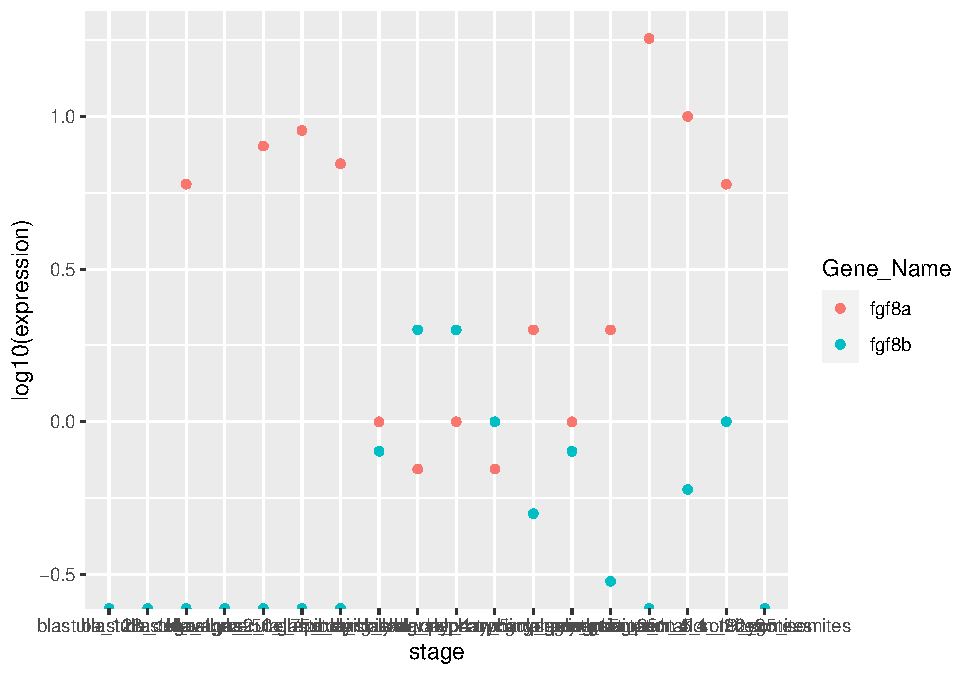
\includegraphics{1_R_basics_and_tidyverse_files/figure-latex/unnamed-chunk-20-1.pdf}

This is ugly, we can make it more readable by: changing the axes names,
changing the orientation of the x-axis text and changing the theme to
remove this grey background. We can also add lines that connect the data
points since it makes sense.

\begin{Shaded}
\begin{Highlighting}[]
\NormalTok{p }\SpecialCharTok{+}
  \FunctionTok{geom\_line}\NormalTok{(}\FunctionTok{aes}\NormalTok{(}\AttributeTok{x =}\NormalTok{ stage, }\AttributeTok{y =} \FunctionTok{log10}\NormalTok{(expression), }\AttributeTok{col =}\NormalTok{ Gene\_Name, }\AttributeTok{group =}\NormalTok{ Gene\_Name)) }\SpecialCharTok{+}
  \FunctionTok{xlab}\NormalTok{(}\StringTok{"Developmental stage"}\NormalTok{) }\SpecialCharTok{+}
  \FunctionTok{ylab}\NormalTok{(}\StringTok{"Log10(FPKM)"}\NormalTok{) }\SpecialCharTok{+}
  \FunctionTok{theme\_classic}\NormalTok{() }\SpecialCharTok{+}
  \FunctionTok{theme}\NormalTok{(}\AttributeTok{axis.text.x =} \FunctionTok{element\_text}\NormalTok{(}\AttributeTok{angle =} \DecValTok{45}\NormalTok{, }\AttributeTok{hjust =} \DecValTok{1}\NormalTok{))}
\end{Highlighting}
\end{Shaded}

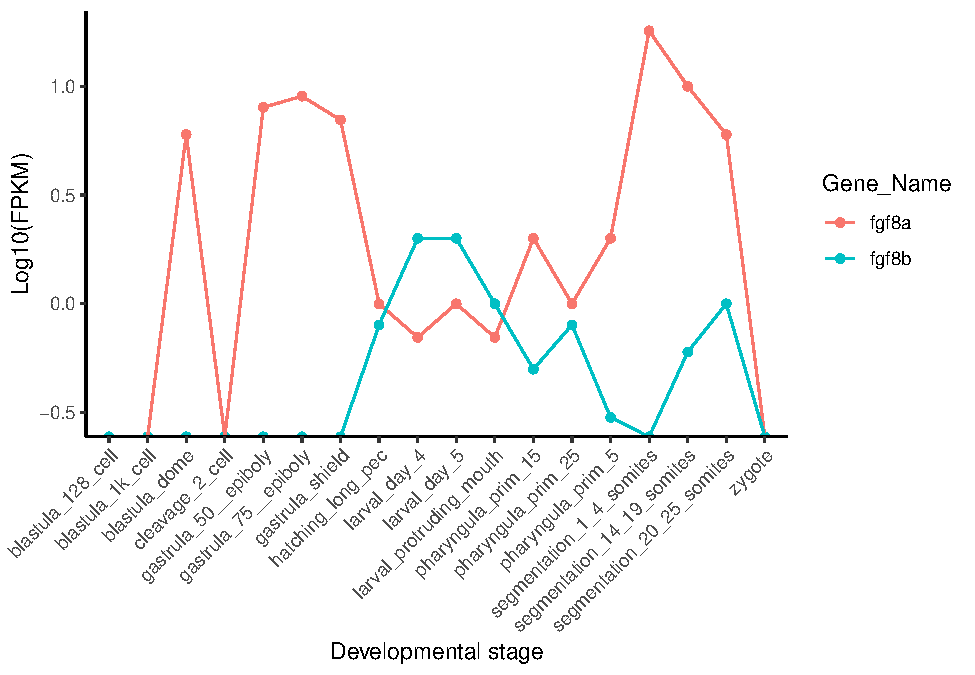
\includegraphics{1_R_basics_and_tidyverse_files/figure-latex/unnamed-chunk-21-1.pdf}
One thing to notice here is that the order of the developmental stages
is messed up. This is because, depending on what method you use to
convert the wide format to the long format, the order of the column may
or may not be preserved (this is why \texttt{reshape2::melt()} is
superior). Here, the \texttt{tidyr} functions reorder the variables by
alphabetical order.

One simple way to deal with this is to manual add levels to the
\texttt{stage} column (factor):

\begin{Shaded}
\begin{Highlighting}[]
\NormalTok{count\_table\_long }\OtherTok{\textless{}{-}}\NormalTok{ count\_table\_long }\SpecialCharTok{\%\textgreater{}\%} 
  \FunctionTok{mutate}\NormalTok{(}\AttributeTok{stage =} \FunctionTok{factor}\NormalTok{(stage, }\AttributeTok{levels =} \FunctionTok{colnames}\NormalTok{(count\_table)[}\SpecialCharTok{{-}}\DecValTok{1}\NormalTok{]))}
\end{Highlighting}
\end{Shaded}

Effectively, we are extracting the stage names in the proper order from
the column names of the count table (\texttt{{[}-1{]}} removes the
\texttt{Gene\_Name} column) and specifying them into the
\texttt{factor()} function.

Let's try to plot it again:

\begin{Shaded}
\begin{Highlighting}[]
\NormalTok{count\_table\_long }\SpecialCharTok{\%\textgreater{}\%} 
  \FunctionTok{filter}\NormalTok{(Gene\_Name }\SpecialCharTok{\%in\%} \FunctionTok{c}\NormalTok{(}\StringTok{"fgf8a"}\NormalTok{, }\StringTok{"fgf8b"}\NormalTok{)) }\SpecialCharTok{\%\textgreater{}\%}
  \FunctionTok{mutate}\NormalTok{(}\AttributeTok{expression =} \FunctionTok{log10}\NormalTok{(expression)) }\SpecialCharTok{\%\textgreater{}\%} 
  \FunctionTok{ggplot}\NormalTok{() }\SpecialCharTok{+}
  \FunctionTok{geom\_point}\NormalTok{(}\FunctionTok{aes}\NormalTok{(}\AttributeTok{x =}\NormalTok{ stage, }\AttributeTok{y =}\NormalTok{ expression, }\AttributeTok{col =}\NormalTok{ Gene\_Name)) }\SpecialCharTok{+}
  \FunctionTok{geom\_line}\NormalTok{(}\FunctionTok{aes}\NormalTok{(}\AttributeTok{x =}\NormalTok{ stage, }\AttributeTok{y =}\NormalTok{ expression, }\AttributeTok{col =}\NormalTok{ Gene\_Name, }\AttributeTok{group =}\NormalTok{ Gene\_Name)) }\SpecialCharTok{+}
  \FunctionTok{xlab}\NormalTok{(}\StringTok{"Developmental stage"}\NormalTok{) }\SpecialCharTok{+}
  \FunctionTok{ylab}\NormalTok{(}\StringTok{"Log10(FPKM)"}\NormalTok{) }\SpecialCharTok{+}
  \FunctionTok{theme\_classic}\NormalTok{() }\SpecialCharTok{+}
  \FunctionTok{theme}\NormalTok{(}\AttributeTok{axis.text.x =} \FunctionTok{element\_text}\NormalTok{(}\AttributeTok{angle =} \DecValTok{45}\NormalTok{, }\AttributeTok{hjust =} \DecValTok{1}\NormalTok{)) }\SpecialCharTok{+}
  \FunctionTok{scale\_color\_manual}\NormalTok{(}\AttributeTok{values =} \FunctionTok{c}\NormalTok{(}\StringTok{"goldenrod"}\NormalTok{, }\StringTok{"royalblue"}\NormalTok{)) }
\end{Highlighting}
\end{Shaded}

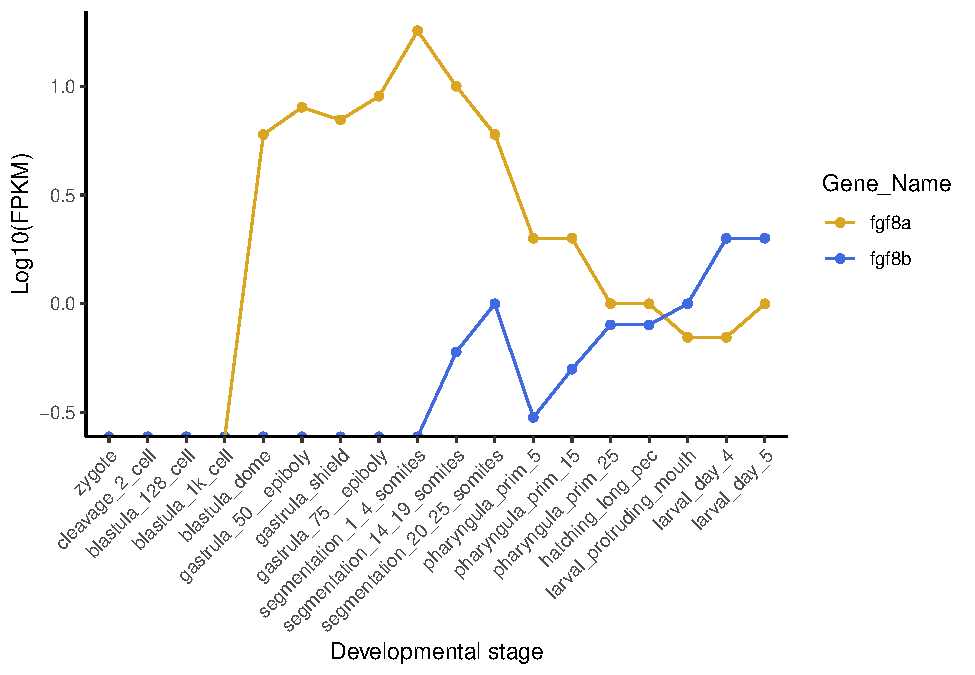
\includegraphics{1_R_basics_and_tidyverse_files/figure-latex/unnamed-chunk-23-1.pdf}

\begin{Shaded}
\begin{Highlighting}[]
\CommentTok{\# Changing the colors, the other ones are horrible}
\end{Highlighting}
\end{Shaded}

There are other things that we could do to make the plot look better
(for instance, changing the name of the developmental stages to get rid
of the \texttt{\_}), but it's fine for now. :)

\end{document}
